
\section{Diagrama de Atividades}
Este capítulo dedica-se a explanar como a aplicação proposta para a intervenção ao problema, anteriormente descrito, executa suas ações e interações, fluxo de ação entre atividades e interçãocom outras aplicações. Para isso, é mostrado os fluxos e atividades de suas ações em figuras e descrito detalhadamente o que pode ser extraído das imagens.

O intuito utilizar-se do Diagrama de Atividades é dar ênfase ao fluxo de controle na execução de um comportamento realizado por um sistema, mostrando o fluxo entre atividades em um sistemas. As atividades podem ser referidas como um fluxo sequencial ou ramificação de atividades que interagem entre si e outros objetos para realizar ou sofrer ações. Descrevendo assim, uma modelagens a função do sistema \cite{Booch:2012}.  

Ao iniciar aplicação é apresentada a tela inicial contendo um campo para entrada de dados para a pesquisa e botões de escolha. Este campo é utilizado para a entrada da sentença em linguagem natural para busca do usuário que esta utilizando a aplicação. 


\begin{figure}[!htb]
        \caption{\label{diagact}Diagrama de Atividade}
        \begin{center}
                \includegraphics[width=\textwidth]{imagens/diagact.eps}
        \end{center}
        \legend{Fonte: Autor}
\end{figure}

\newpage
\section{Fluxo de funcionamento da aplicação}
\lipsum[3-7]

\begin{figure}[!htb]
        \caption{\label{diagfluxo}Fluxo de funcionamento da aplicação}
        \begin{center}
                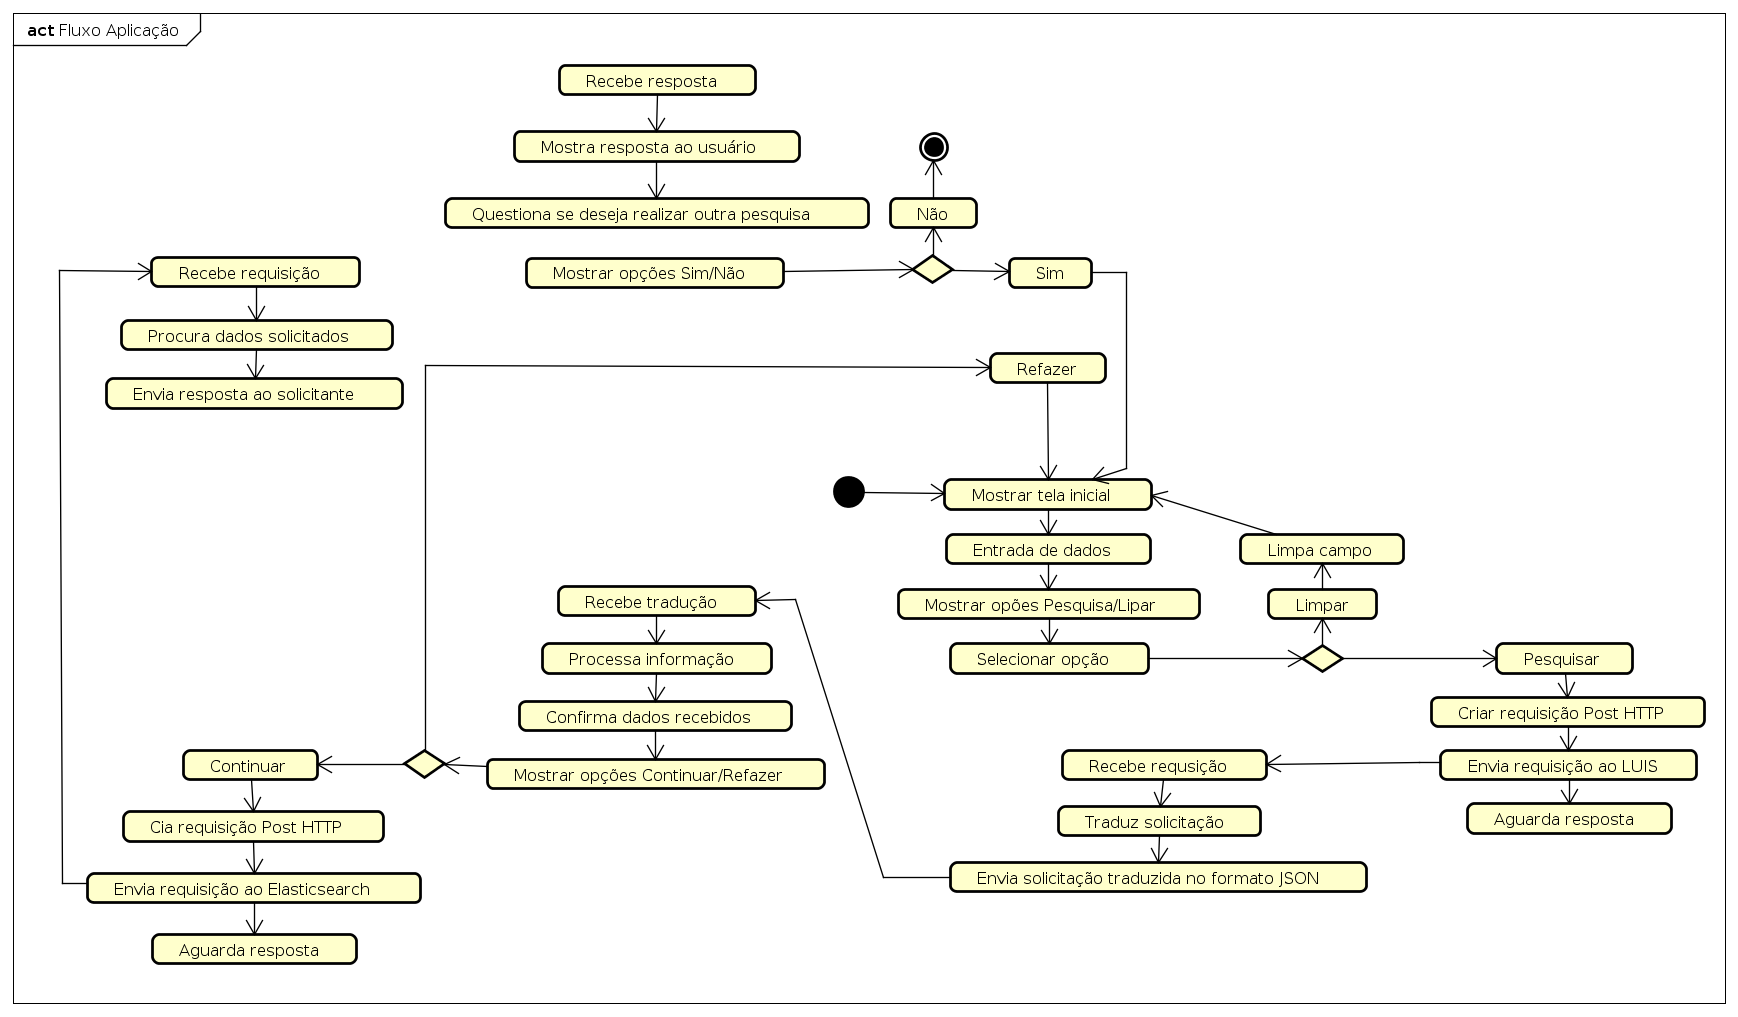
\includegraphics[angle=90, width=\textwidth, height=\textheight]{imagens/diagfluxo.eps}
        \end{center}
        \legend{Fonte: Autor}
\end{figure}
